
    % latexmk -pdflatex='lualatex' -pdf FontExhibition.tex
    \documentclass[parskip,landscape,letter]{scrartcl}
    \usepackage{fontspec}
    \usepackage[margin=10mm,left=20mm]{geometry}
    \usepackage{tikz}
    \usetikzlibrary{matrix,backgrounds}
    \usepackage{pifont}
    \usepackage{graphicx}
    \usepackage{chessfss}
    \usepackage{setspace}
    \usepackage{enumitem}
    \usepackage{amssymb}
    \usepackage{graphicx,calc}
    \graphicspath{{./graphics/}}
    \input{symbols.tex}

    \begin{document}
    \setmainfont[Extension={.ttf},ItalicFont={DejaVuSerif-Italic}]{FreeSerif}
    
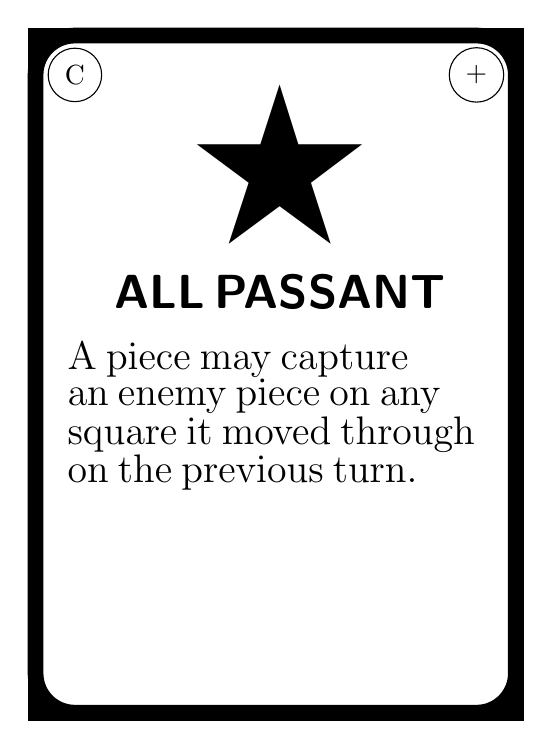
\begin{tikzpicture}
    \pgfmathsetmacro{\cardroundingradius}{5mm}
    \pgfmathsetmacro{\striproundingradius}{3mm}
    % \pgfmathsetmacro{\cardwidth}{5.9}
    % \pgfmathsetmacro{\cardheight}{9.2}
    \pgfmathsetmacro{\cardwidth}{6.1}  % Magic cards are 63x88mm
    \pgfmathsetmacro{\cardheight}{8.6}
    \pgfmathsetmacro{\stripwidth}{1.2}
    \pgfmathsetmacro{\strippadding}{0.1}
    \pgfmathsetmacro{\textpadding}{0.3}
    \pgfmathsetmacro{\ruleheight}{0.1}
    \providecommand{\stripfontsize}{\Huge}
    \providecommand{\captionfontsize}{\LARGE}
    \providecommand{\textfontsize}{\Large}
    \providecommand{\quotefontsize}{\small}
    \draw[fill=white, line width=2mm,rounded corners=\cardroundingradius] (0,0) rectangle (\cardwidth,\cardheight);
    \draw[line width=2mm] (0,0) rectangle (\cardwidth,\cardheight);
    \node[text width=(\cardwidth-\strippadding-2*\textpadding)*1cm,below right,inner sep=0] at (\strippadding+\textpadding,\cardheight-\textpadding) 
    { 
    \begin{center} {\fontsize{80pt}{60pt}\selectfont \ding{72}}\\\end{center}
\begin{center}
    {\captionfontsize \textsf{\textbf{ALL PASSANT}}}\end{center}
        {\textfontsize A piece may capture an enemy piece on any square it moved through on the previous turn.}
        %\tikz{\fill (0,0) rectangle (\cardwidth-2*\strippadding-2*\textpadding,\ruleheight);}\\
        {\quotefontsize \textit{}}\\[-2\baselineskip]
    };
    \node[circle,draw,text=black](c) at (.5,\cardheight-.5){C};
    \node[circle,draw,text=black](c) at (\cardwidth-.5,\cardheight-.5){+};
    \end{tikzpicture}%
\hspace{1pt}%
\begin{tikzpicture}
    \pgfmathsetmacro{\cardroundingradius}{5mm}
    \pgfmathsetmacro{\striproundingradius}{3mm}
    % \pgfmathsetmacro{\cardwidth}{5.9}
    % \pgfmathsetmacro{\cardheight}{9.2}
    \pgfmathsetmacro{\cardwidth}{6.1}  % Magic cards are 63x88mm
    \pgfmathsetmacro{\cardheight}{8.6}
    \pgfmathsetmacro{\stripwidth}{1.2}
    \pgfmathsetmacro{\strippadding}{0.1}
    \pgfmathsetmacro{\textpadding}{0.3}
    \pgfmathsetmacro{\ruleheight}{0.1}
    \providecommand{\stripfontsize}{\Huge}
    \providecommand{\captionfontsize}{\LARGE}
    \providecommand{\textfontsize}{\Large}
    \providecommand{\quotefontsize}{\small}
    \draw[fill=white, line width=2mm,rounded corners=\cardroundingradius] (0,0) rectangle (\cardwidth,\cardheight);
    \draw[line width=2mm] (0,0) rectangle (\cardwidth,\cardheight);
    \node[text width=(\cardwidth-\strippadding-2*\textpadding)*1cm,below right,inner sep=0] at (\strippadding+\textpadding,\cardheight-\textpadding) 
    { 
    \begin{center} {\fontsize{80pt}{60pt}\selectfont \Bishop\Knight}\\\end{center}
\begin{center}
    {\captionfontsize \textsf{\textbf{BISHOP KNIGHT SWAP}}}\end{center}
        {\textfontsize A \Bishop\ moves like a \Bishop, but captures only like a \Knight. A \Knight\ moves like a \Knight, but captures only like a \Bishop.}
        %\tikz{\fill (0,0) rectangle (\cardwidth-2*\strippadding-2*\textpadding,\ruleheight);}\\
        {\quotefontsize \textit{}}\\[-2\baselineskip]
    };
    \node[circle,draw,text=black](c) at (.5,\cardheight-.5){C};
    \node[circle,draw,text=black](c) at (\cardwidth-.5,\cardheight-.5){\diff};
    \end{tikzpicture}%
\hspace{1pt}%
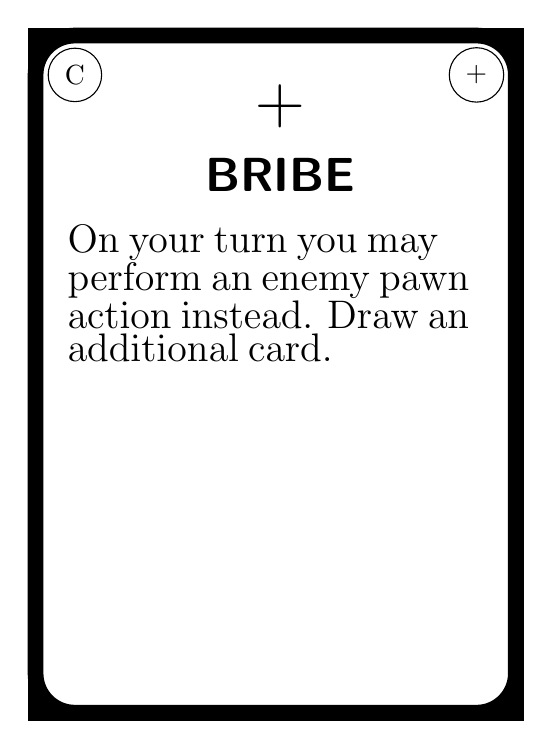
\begin{tikzpicture}
    \pgfmathsetmacro{\cardroundingradius}{5mm}
    \pgfmathsetmacro{\striproundingradius}{3mm}
    % \pgfmathsetmacro{\cardwidth}{5.9}
    % \pgfmathsetmacro{\cardheight}{9.2}
    \pgfmathsetmacro{\cardwidth}{6.1}  % Magic cards are 63x88mm
    \pgfmathsetmacro{\cardheight}{8.6}
    \pgfmathsetmacro{\stripwidth}{1.2}
    \pgfmathsetmacro{\strippadding}{0.1}
    \pgfmathsetmacro{\textpadding}{0.3}
    \pgfmathsetmacro{\ruleheight}{0.1}
    \providecommand{\stripfontsize}{\Huge}
    \providecommand{\captionfontsize}{\LARGE}
    \providecommand{\textfontsize}{\Large}
    \providecommand{\quotefontsize}{\small}
    \draw[fill=white, line width=2mm,rounded corners=\cardroundingradius] (0,0) rectangle (\cardwidth,\cardheight);
    \draw[line width=2mm] (0,0) rectangle (\cardwidth,\cardheight);
    \node[text width=(\cardwidth-\strippadding-2*\textpadding)*1cm,below right,inner sep=0] at (\strippadding+\textpadding,\cardheight-\textpadding) 
    { 
    \begin{center} {\fontsize{80pt}{60pt}\selectfont \Pawn+}\\\end{center}
\begin{center}
    {\captionfontsize \textsf{\textbf{BRIBE}}}\end{center}
        {\textfontsize On your turn you may perform an enemy pawn action instead. Draw an additional card.}
        %\tikz{\fill (0,0) rectangle (\cardwidth-2*\strippadding-2*\textpadding,\ruleheight);}\\
        {\quotefontsize \textit{}}\\[-2\baselineskip]
    };
    \node[circle,draw,text=black](c) at (.5,\cardheight-.5){C};
    \node[circle,draw,text=black](c) at (\cardwidth-.5,\cardheight-.5){+};
    \end{tikzpicture}%
\hspace{1pt}%
\begin{tikzpicture}
    \pgfmathsetmacro{\cardroundingradius}{5mm}
    \pgfmathsetmacro{\striproundingradius}{3mm}
    % \pgfmathsetmacro{\cardwidth}{5.9}
    % \pgfmathsetmacro{\cardheight}{9.2}
    \pgfmathsetmacro{\cardwidth}{6.1}  % Magic cards are 63x88mm
    \pgfmathsetmacro{\cardheight}{8.6}
    \pgfmathsetmacro{\stripwidth}{1.2}
    \pgfmathsetmacro{\strippadding}{0.1}
    \pgfmathsetmacro{\textpadding}{0.3}
    \pgfmathsetmacro{\ruleheight}{0.1}
    \providecommand{\stripfontsize}{\Huge}
    \providecommand{\captionfontsize}{\LARGE}
    \providecommand{\textfontsize}{\Large}
    \providecommand{\quotefontsize}{\small}
    \draw[fill=white, line width=2mm,rounded corners=\cardroundingradius] (0,0) rectangle (\cardwidth,\cardheight);
    \draw[line width=2mm] (0,0) rectangle (\cardwidth,\cardheight);
    \node[text width=(\cardwidth-\strippadding-2*\textpadding)*1cm,below right,inner sep=0] at (\strippadding+\textpadding,\cardheight-\textpadding) 
    { 
    \begin{center} {\fontsize{80pt}{60pt}\selectfont \KI\KII}\\\end{center}
\begin{center}
    {\captionfontsize \textsf{\textbf{CAPTURE SWAP}}}\end{center}
        {\textfontsize An X moves like an X, but captures only like a Y. A Y moves like a Y, but captures only like an X.}
        %\tikz{\fill (0,0) rectangle (\cardwidth-2*\strippadding-2*\textpadding,\ruleheight);}\\
        {\quotefontsize \textit{}}\\[-2\baselineskip]
    };
    \node[circle,draw,text=black](c) at (.5,\cardheight-.5){C};
    \node[circle,draw,text=black](c) at (\cardwidth-.5,\cardheight-.5){\diff};
    \end{tikzpicture}%
\hspace{1pt}%
\\[-.5\lineskip]
\begin{tikzpicture}
    \pgfmathsetmacro{\cardroundingradius}{5mm}
    \pgfmathsetmacro{\striproundingradius}{3mm}
    % \pgfmathsetmacro{\cardwidth}{5.9}
    % \pgfmathsetmacro{\cardheight}{9.2}
    \pgfmathsetmacro{\cardwidth}{6.1}  % Magic cards are 63x88mm
    \pgfmathsetmacro{\cardheight}{8.6}
    \pgfmathsetmacro{\stripwidth}{1.2}
    \pgfmathsetmacro{\strippadding}{0.1}
    \pgfmathsetmacro{\textpadding}{0.3}
    \pgfmathsetmacro{\ruleheight}{0.1}
    \providecommand{\stripfontsize}{\Huge}
    \providecommand{\captionfontsize}{\LARGE}
    \providecommand{\textfontsize}{\Large}
    \providecommand{\quotefontsize}{\small}
    \draw[fill=white, line width=2mm,rounded corners=\cardroundingradius] (0,0) rectangle (\cardwidth,\cardheight);
    \draw[line width=2mm] (0,0) rectangle (\cardwidth,\cardheight);
    \node[text width=(\cardwidth-\strippadding-2*\textpadding)*1cm,below right,inner sep=0] at (\strippadding+\textpadding,\cardheight-\textpadding) 
    { 
    \begin{center} {\fontsize{80pt}{60pt}\selectfont \All}\\\end{center}
\begin{center}
    {\captionfontsize \textsf{\textbf{CAPTURE TWICE}}}\end{center}
        {\textfontsize You may make two captures with two different pieces as one action.}
        %\tikz{\fill (0,0) rectangle (\cardwidth-2*\strippadding-2*\textpadding,\ruleheight);}\\
        {\quotefontsize \textit{}}\\[-2\baselineskip]
    };
    \node[circle,draw,text=black](c) at (.5,\cardheight-.5){C};
    \node[circle,draw,text=black](c) at (\cardwidth-.5,\cardheight-.5){+};
    \end{tikzpicture}%
\hspace{1pt}%
\begin{tikzpicture}
    \pgfmathsetmacro{\cardroundingradius}{5mm}
    \pgfmathsetmacro{\striproundingradius}{3mm}
    % \pgfmathsetmacro{\cardwidth}{5.9}
    % \pgfmathsetmacro{\cardheight}{9.2}
    \pgfmathsetmacro{\cardwidth}{6.1}  % Magic cards are 63x88mm
    \pgfmathsetmacro{\cardheight}{8.6}
    \pgfmathsetmacro{\stripwidth}{1.2}
    \pgfmathsetmacro{\strippadding}{0.1}
    \pgfmathsetmacro{\textpadding}{0.3}
    \pgfmathsetmacro{\ruleheight}{0.1}
    \providecommand{\stripfontsize}{\Huge}
    \providecommand{\captionfontsize}{\LARGE}
    \providecommand{\textfontsize}{\Large}
    \providecommand{\quotefontsize}{\small}
    \draw[fill=white, line width=2mm,rounded corners=\cardroundingradius] (0,0) rectangle (\cardwidth,\cardheight);
    \draw[line width=2mm] (0,0) rectangle (\cardwidth,\cardheight);
    \node[text width=(\cardwidth-\strippadding-2*\textpadding)*1cm,below right,inner sep=0] at (\strippadding+\textpadding,\cardheight-\textpadding) 
    { 
    \begin{center} {\fontsize{80pt}{60pt}\selectfont \NoKing}\\\end{center}
\begin{center}
    {\captionfontsize \textsf{\textbf{CASTLES FOR EVERYONE}}}\end{center}
        {\textfontsize \small Any \NoKing\ X may castle with a friendly \NoKing\ Y on the same rank or file. X jumps two squares towards (or over or onto) Y and Y moves to the square X jumped over.}
        %\tikz{\fill (0,0) rectangle (\cardwidth-2*\strippadding-2*\textpadding,\ruleheight);}\\
        {\quotefontsize \textit{}}\\[-2\baselineskip]
    };
    \node[circle,draw,text=black](c) at (.5,\cardheight-.5){C};
    \node[circle,draw,text=black](c) at (\cardwidth-.5,\cardheight-.5){+};
    \end{tikzpicture}%
\hspace{1pt}%
\begin{tikzpicture}
    \pgfmathsetmacro{\cardroundingradius}{5mm}
    \pgfmathsetmacro{\striproundingradius}{3mm}
    % \pgfmathsetmacro{\cardwidth}{5.9}
    % \pgfmathsetmacro{\cardheight}{9.2}
    \pgfmathsetmacro{\cardwidth}{6.1}  % Magic cards are 63x88mm
    \pgfmathsetmacro{\cardheight}{8.6}
    \pgfmathsetmacro{\stripwidth}{1.2}
    \pgfmathsetmacro{\strippadding}{0.1}
    \pgfmathsetmacro{\textpadding}{0.3}
    \pgfmathsetmacro{\ruleheight}{0.1}
    \providecommand{\stripfontsize}{\Huge}
    \providecommand{\captionfontsize}{\LARGE}
    \providecommand{\textfontsize}{\Large}
    \providecommand{\quotefontsize}{\small}
    \draw[fill=white, line width=2mm,rounded corners=\cardroundingradius] (0,0) rectangle (\cardwidth,\cardheight);
    \draw[line width=2mm] (0,0) rectangle (\cardwidth,\cardheight);
    \node[text width=(\cardwidth-\strippadding-2*\textpadding)*1cm,below right,inner sep=0] at (\strippadding+\textpadding,\cardheight-\textpadding) 
    { 
    \begin{center} {\fontsize{80pt}{60pt}\selectfont \King\Knight}\\\end{center}
\begin{center}
    {\captionfontsize \textsf{\textbf{KING KNIGHT SWAP}}}\end{center}
        {\textfontsize A \King\ acts only like a \Knight. A \Knight\ acts only like a \King.}
        %\tikz{\fill (0,0) rectangle (\cardwidth-2*\strippadding-2*\textpadding,\ruleheight);}\\
        {\quotefontsize \textit{}}\\[-2\baselineskip]
    };
    \node[circle,draw,text=black](c) at (.5,\cardheight-.5){C};
    \node[circle,draw,text=black](c) at (\cardwidth-.5,\cardheight-.5){\diff};
    \end{tikzpicture}%
\hspace{1pt}%
\begin{tikzpicture}
    \pgfmathsetmacro{\cardroundingradius}{5mm}
    \pgfmathsetmacro{\striproundingradius}{3mm}
    % \pgfmathsetmacro{\cardwidth}{5.9}
    % \pgfmathsetmacro{\cardheight}{9.2}
    \pgfmathsetmacro{\cardwidth}{6.1}  % Magic cards are 63x88mm
    \pgfmathsetmacro{\cardheight}{8.6}
    \pgfmathsetmacro{\stripwidth}{1.2}
    \pgfmathsetmacro{\strippadding}{0.1}
    \pgfmathsetmacro{\textpadding}{0.3}
    \pgfmathsetmacro{\ruleheight}{0.1}
    \providecommand{\stripfontsize}{\Huge}
    \providecommand{\captionfontsize}{\LARGE}
    \providecommand{\textfontsize}{\Large}
    \providecommand{\quotefontsize}{\small}
    \draw[fill=white, line width=2mm,rounded corners=\cardroundingradius] (0,0) rectangle (\cardwidth,\cardheight);
    \draw[line width=2mm] (0,0) rectangle (\cardwidth,\cardheight);
    \node[text width=(\cardwidth-\strippadding-2*\textpadding)*1cm,below right,inner sep=0] at (\strippadding+\textpadding,\cardheight-\textpadding) 
    { 
    \begin{center} {\fontsize{80pt}{60pt}\selectfont \Queen\Rook}\\\end{center}
\begin{center}
    {\captionfontsize \textsf{\textbf{QUEEN ROOK SWAP}}}\end{center}
        {\textfontsize A \Queen\ moves like a \Queen, but captures only like a \Rook. A \Rook\ moves like a \Rook, but captures only like a \Queen.}
        %\tikz{\fill (0,0) rectangle (\cardwidth-2*\strippadding-2*\textpadding,\ruleheight);}\\
        {\quotefontsize \textit{}}\\[-2\baselineskip]
    };
    \node[circle,draw,text=black](c) at (.5,\cardheight-.5){C};
    \node[circle,draw,text=black](c) at (\cardwidth-.5,\cardheight-.5){\diff};
    \end{tikzpicture}%
\hspace{1pt}%
\\[-.5\lineskip]
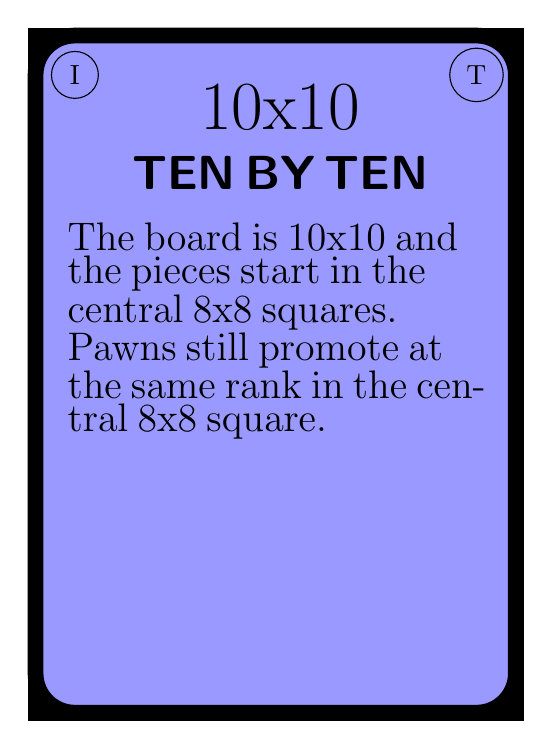
\begin{tikzpicture}
    \pgfmathsetmacro{\cardroundingradius}{5mm}
    \pgfmathsetmacro{\striproundingradius}{3mm}
    % \pgfmathsetmacro{\cardwidth}{5.9}
    % \pgfmathsetmacro{\cardheight}{9.2}
    \pgfmathsetmacro{\cardwidth}{6.1}  % Magic cards are 63x88mm
    \pgfmathsetmacro{\cardheight}{8.6}
    \pgfmathsetmacro{\stripwidth}{1.2}
    \pgfmathsetmacro{\strippadding}{0.1}
    \pgfmathsetmacro{\textpadding}{0.3}
    \pgfmathsetmacro{\ruleheight}{0.1}
    \providecommand{\stripfontsize}{\Huge}
    \providecommand{\captionfontsize}{\LARGE}
    \providecommand{\textfontsize}{\Large}
    \providecommand{\quotefontsize}{\small}
    \draw[fill=blue!40!white, line width=2mm,rounded corners=\cardroundingradius] (0,0) rectangle (\cardwidth,\cardheight);
    \draw[line width=2mm] (0,0) rectangle (\cardwidth,\cardheight);
    \node[text width=(\cardwidth-\strippadding-2*\textpadding)*1cm,below right,inner sep=0] at (\strippadding+\textpadding,\cardheight-\textpadding) 
    { 
    \begin{center} {\fontsize{80pt}{60pt}\selectfont \inlinegraphics{10x10}}\\\end{center}
\begin{center}
    {\captionfontsize \textsf{\textbf{TEN BY TEN}}}\end{center}
        {\textfontsize The board is 10x10 and the pieces start in the central 8x8 squares. Pawns still promote at the same rank in the central 8x8 square.}
        %\tikz{\fill (0,0) rectangle (\cardwidth-2*\strippadding-2*\textpadding,\ruleheight);}\\
        {\quotefontsize \textit{}}\\[-2\baselineskip]
    };
    \node[circle,draw,text=black](c) at (.5,\cardheight-.5){I};
    \node[circle,draw,text=black](c) at (\cardwidth-.5,\cardheight-.5){T};
    \end{tikzpicture}%
\hspace{1pt}%
\begin{tikzpicture}
    \pgfmathsetmacro{\cardroundingradius}{5mm}
    \pgfmathsetmacro{\striproundingradius}{3mm}
    % \pgfmathsetmacro{\cardwidth}{5.9}
    % \pgfmathsetmacro{\cardheight}{9.2}
    \pgfmathsetmacro{\cardwidth}{6.1}  % Magic cards are 63x88mm
    \pgfmathsetmacro{\cardheight}{8.6}
    \pgfmathsetmacro{\stripwidth}{1.2}
    \pgfmathsetmacro{\strippadding}{0.1}
    \pgfmathsetmacro{\textpadding}{0.3}
    \pgfmathsetmacro{\ruleheight}{0.1}
    \providecommand{\stripfontsize}{\Huge}
    \providecommand{\captionfontsize}{\LARGE}
    \providecommand{\textfontsize}{\Large}
    \providecommand{\quotefontsize}{\small}
    \draw[fill=blue!40!white, line width=2mm,rounded corners=\cardroundingradius] (0,0) rectangle (\cardwidth,\cardheight);
    \draw[line width=2mm] (0,0) rectangle (\cardwidth,\cardheight);
    \node[text width=(\cardwidth-\strippadding-2*\textpadding)*1cm,below right,inner sep=0] at (\strippadding+\textpadding,\cardheight-\textpadding) 
    { 
    \begin{center} {\fontsize{80pt}{60pt}\selectfont \All}\\\end{center}
\begin{center}
    {\captionfontsize \textsf{\textbf{MICRO-MANAGER}}}\end{center}
        {\textfontsize Pieces more than one rank in front of the King may not capture.}
        %\tikz{\fill (0,0) rectangle (\cardwidth-2*\strippadding-2*\textpadding,\ruleheight);}\\
        {\quotefontsize \textit{}}\\[-2\baselineskip]
    };
    \node[circle,draw,text=black](c) at (.5,\cardheight-.5){C};
    \node[circle,draw,text=black](c) at (\cardwidth-.5,\cardheight-.5){T};
    \end{tikzpicture}%
\hspace{1pt}%
\begin{tikzpicture}
    \pgfmathsetmacro{\cardroundingradius}{5mm}
    \pgfmathsetmacro{\striproundingradius}{3mm}
    % \pgfmathsetmacro{\cardwidth}{5.9}
    % \pgfmathsetmacro{\cardheight}{9.2}
    \pgfmathsetmacro{\cardwidth}{6.1}  % Magic cards are 63x88mm
    \pgfmathsetmacro{\cardheight}{8.6}
    \pgfmathsetmacro{\stripwidth}{1.2}
    \pgfmathsetmacro{\strippadding}{0.1}
    \pgfmathsetmacro{\textpadding}{0.3}
    \pgfmathsetmacro{\ruleheight}{0.1}
    \providecommand{\stripfontsize}{\Huge}
    \providecommand{\captionfontsize}{\LARGE}
    \providecommand{\textfontsize}{\Large}
    \providecommand{\quotefontsize}{\small}
    \draw[fill=white, line width=2mm,rounded corners=\cardroundingradius] (0,0) rectangle (\cardwidth,\cardheight);
    \draw[line width=2mm] (0,0) rectangle (\cardwidth,\cardheight);
    \node[text width=(\cardwidth-\strippadding-2*\textpadding)*1cm,below right,inner sep=0] at (\strippadding+\textpadding,\cardheight-\textpadding) 
    { 
    \begin{center} {\fontsize{80pt}{60pt}\selectfont \All}\\\end{center}
\begin{center}
    {\captionfontsize \textsf{\textbf{WAR AND PEACE}}}\end{center}
        {\textfontsize You may move and capture with two different pieces as one action.}
        %\tikz{\fill (0,0) rectangle (\cardwidth-2*\strippadding-2*\textpadding,\ruleheight);}\\
        {\quotefontsize \textit{}}\\[-2\baselineskip]
    };
    \node[circle,draw,text=black](c) at (.5,\cardheight-.5){C};
    \node[circle,draw,text=black](c) at (\cardwidth-.5,\cardheight-.5){+};
    \end{tikzpicture}%
\hspace{1pt}%
\begin{tikzpicture}
    \pgfmathsetmacro{\cardroundingradius}{5mm}
    \pgfmathsetmacro{\striproundingradius}{3mm}
    % \pgfmathsetmacro{\cardwidth}{5.9}
    % \pgfmathsetmacro{\cardheight}{9.2}
    \pgfmathsetmacro{\cardwidth}{6.1}  % Magic cards are 63x88mm
    \pgfmathsetmacro{\cardheight}{8.6}
    \pgfmathsetmacro{\stripwidth}{1.2}
    \pgfmathsetmacro{\strippadding}{0.1}
    \pgfmathsetmacro{\textpadding}{0.3}
    \pgfmathsetmacro{\ruleheight}{0.1}
    \providecommand{\stripfontsize}{\Huge}
    \providecommand{\captionfontsize}{\LARGE}
    \providecommand{\textfontsize}{\Large}
    \providecommand{\quotefontsize}{\small}
    \draw[fill=white, line width=2mm,rounded corners=\cardroundingradius] (0,0) rectangle (\cardwidth,\cardheight);
    \draw[line width=2mm] (0,0) rectangle (\cardwidth,\cardheight);
    \node[text width=(\cardwidth-\strippadding-2*\textpadding)*1cm,below right,inner sep=0] at (\strippadding+\textpadding,\cardheight-\textpadding) 
    { 
    \begin{center} {\fontsize{80pt}{60pt}\selectfont \NoKing}\\\end{center}
\begin{center}
    {\captionfontsize \textsf{\textbf{KNIGHT SWAP}}}\end{center}
        {\textfontsize Two friendly \NoKing\ pieces which are a knight move apart may swap places as an action.}
        %\tikz{\fill (0,0) rectangle (\cardwidth-2*\strippadding-2*\textpadding,\ruleheight);}\\
        {\quotefontsize \textit{}}\\[-2\baselineskip]
    };
    \node[circle,draw,text=black](c) at (.5,\cardheight-.5){C};
    \node[circle,draw,text=black](c) at (\cardwidth-.5,\cardheight-.5){+};
    \end{tikzpicture}%
\hspace{1pt}%
\\[-.5\lineskip]
\begin{tikzpicture}
    \pgfmathsetmacro{\cardroundingradius}{5mm}
    \pgfmathsetmacro{\striproundingradius}{3mm}
    % \pgfmathsetmacro{\cardwidth}{5.9}
    % \pgfmathsetmacro{\cardheight}{9.2}
    \pgfmathsetmacro{\cardwidth}{6.1}  % Magic cards are 63x88mm
    \pgfmathsetmacro{\cardheight}{8.6}
    \pgfmathsetmacro{\stripwidth}{1.2}
    \pgfmathsetmacro{\strippadding}{0.1}
    \pgfmathsetmacro{\textpadding}{0.3}
    \pgfmathsetmacro{\ruleheight}{0.1}
    \providecommand{\stripfontsize}{\Huge}
    \providecommand{\captionfontsize}{\LARGE}
    \providecommand{\textfontsize}{\Large}
    \providecommand{\quotefontsize}{\small}
    \draw[fill=white, line width=2mm,rounded corners=\cardroundingradius] (0,0) rectangle (\cardwidth,\cardheight);
    \draw[line width=2mm] (0,0) rectangle (\cardwidth,\cardheight);
    \node[text width=(\cardwidth-\strippadding-2*\textpadding)*1cm,below right,inner sep=0] at (\strippadding+\textpadding,\cardheight-\textpadding) 
    { 
    \begin{center} {\fontsize{80pt}{60pt}\selectfont \Bishop}\\\end{center}
\begin{center}
    {\captionfontsize \textsf{\textbf{TELEPORTER}}}\end{center}
        {\textfontsize A \Bishop\ may move to any open square adjacent to a friendly pawn.}
        %\tikz{\fill (0,0) rectangle (\cardwidth-2*\strippadding-2*\textpadding,\ruleheight);}\\
        {\quotefontsize \textit{}}\\[-2\baselineskip]
    };
    \node[circle,draw,text=black](c) at (.5,\cardheight-.5){C};
    \node[circle,draw,text=black](c) at (\cardwidth-.5,\cardheight-.5){+};
    \end{tikzpicture}%
\hspace{1pt}%
\begin{tikzpicture}
    \pgfmathsetmacro{\cardroundingradius}{5mm}
    \pgfmathsetmacro{\striproundingradius}{3mm}
    % \pgfmathsetmacro{\cardwidth}{5.9}
    % \pgfmathsetmacro{\cardheight}{9.2}
    \pgfmathsetmacro{\cardwidth}{6.1}  % Magic cards are 63x88mm
    \pgfmathsetmacro{\cardheight}{8.6}
    \pgfmathsetmacro{\stripwidth}{1.2}
    \pgfmathsetmacro{\strippadding}{0.1}
    \pgfmathsetmacro{\textpadding}{0.3}
    \pgfmathsetmacro{\ruleheight}{0.1}
    \providecommand{\stripfontsize}{\Huge}
    \providecommand{\captionfontsize}{\LARGE}
    \providecommand{\textfontsize}{\Large}
    \providecommand{\quotefontsize}{\small}
    \draw[fill=white, line width=2mm,rounded corners=\cardroundingradius] (0,0) rectangle (\cardwidth,\cardheight);
    \draw[line width=2mm] (0,0) rectangle (\cardwidth,\cardheight);
    \node[text width=(\cardwidth-\strippadding-2*\textpadding)*1cm,below right,inner sep=0] at (\strippadding+\textpadding,\cardheight-\textpadding) 
    { 
    \begin{center} {\fontsize{80pt}{60pt}\selectfont \Bishop}\\\end{center}
\begin{center}
    {\captionfontsize \textsf{\textbf{SUMMONER}}}\end{center}
        {\textfontsize A \Bishop\ may move a friendly \NoKing\ to an adjacent square next to it as an action.}
        %\tikz{\fill (0,0) rectangle (\cardwidth-2*\strippadding-2*\textpadding,\ruleheight);}\\
        {\quotefontsize \textit{}}\\[-2\baselineskip]
    };
    \node[circle,draw,text=black](c) at (.5,\cardheight-.5){C};
    \node[circle,draw,text=black](c) at (\cardwidth-.5,\cardheight-.5){+};
    \end{tikzpicture}%
\hspace{1pt}%
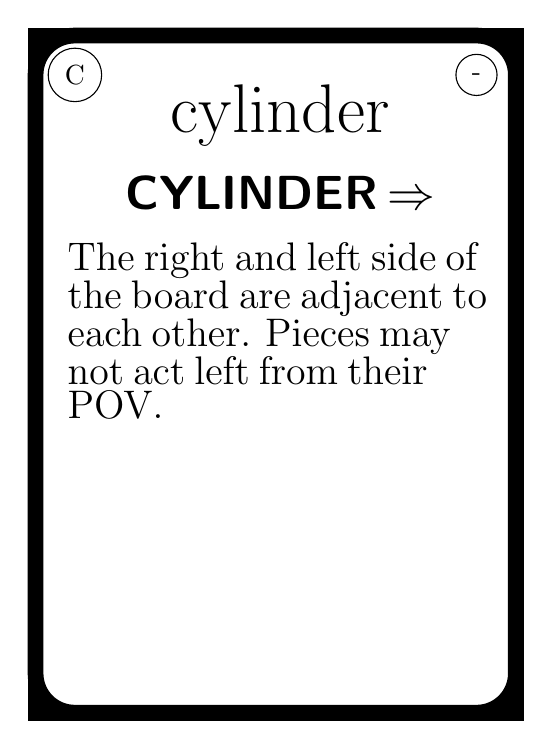
\begin{tikzpicture}
    \pgfmathsetmacro{\cardroundingradius}{5mm}
    \pgfmathsetmacro{\striproundingradius}{3mm}
    % \pgfmathsetmacro{\cardwidth}{5.9}
    % \pgfmathsetmacro{\cardheight}{9.2}
    \pgfmathsetmacro{\cardwidth}{6.1}  % Magic cards are 63x88mm
    \pgfmathsetmacro{\cardheight}{8.6}
    \pgfmathsetmacro{\stripwidth}{1.2}
    \pgfmathsetmacro{\strippadding}{0.1}
    \pgfmathsetmacro{\textpadding}{0.3}
    \pgfmathsetmacro{\ruleheight}{0.1}
    \providecommand{\stripfontsize}{\Huge}
    \providecommand{\captionfontsize}{\LARGE}
    \providecommand{\textfontsize}{\Large}
    \providecommand{\quotefontsize}{\small}
    \draw[fill=white, line width=2mm,rounded corners=\cardroundingradius] (0,0) rectangle (\cardwidth,\cardheight);
    \draw[line width=2mm] (0,0) rectangle (\cardwidth,\cardheight);
    \node[text width=(\cardwidth-\strippadding-2*\textpadding)*1cm,below right,inner sep=0] at (\strippadding+\textpadding,\cardheight-\textpadding) 
    { 
    \begin{center} {\fontsize{80pt}{60pt}\selectfont \inlinegraphics{cylinder}}\\\end{center}
\begin{center}
    {\captionfontsize \textsf{\textbf{CYLINDER $\Rightarrow$}}}\end{center}
        {\textfontsize The right and left side of the board are adjacent to each other. Pieces may not act left from their POV.}
        %\tikz{\fill (0,0) rectangle (\cardwidth-2*\strippadding-2*\textpadding,\ruleheight);}\\
        {\quotefontsize \textit{}}\\[-2\baselineskip]
    };
    \node[circle,draw,text=black](c) at (.5,\cardheight-.5){C};
    \node[circle,draw,text=black](c) at (\cardwidth-.5,\cardheight-.5){-};
    \end{tikzpicture}%
\hspace{1pt}%
\begin{tikzpicture}
    \pgfmathsetmacro{\cardroundingradius}{5mm}
    \pgfmathsetmacro{\striproundingradius}{3mm}
    % \pgfmathsetmacro{\cardwidth}{5.9}
    % \pgfmathsetmacro{\cardheight}{9.2}
    \pgfmathsetmacro{\cardwidth}{6.1}  % Magic cards are 63x88mm
    \pgfmathsetmacro{\cardheight}{8.6}
    \pgfmathsetmacro{\stripwidth}{1.2}
    \pgfmathsetmacro{\strippadding}{0.1}
    \pgfmathsetmacro{\textpadding}{0.3}
    \pgfmathsetmacro{\ruleheight}{0.1}
    \providecommand{\stripfontsize}{\Huge}
    \providecommand{\captionfontsize}{\LARGE}
    \providecommand{\textfontsize}{\Large}
    \providecommand{\quotefontsize}{\small}
    \draw[fill=white, line width=2mm,rounded corners=\cardroundingradius] (0,0) rectangle (\cardwidth,\cardheight);
    \draw[line width=2mm] (0,0) rectangle (\cardwidth,\cardheight);
    \node[text width=(\cardwidth-\strippadding-2*\textpadding)*1cm,below right,inner sep=0] at (\strippadding+\textpadding,\cardheight-\textpadding) 
    { 
    \begin{center} {\fontsize{80pt}{60pt}\selectfont \Knight\Pawn}\\\end{center}
\begin{center}
    {\captionfontsize \textsf{\textbf{TRADING PLACES}}}\end{center}
        {\textfontsize You may swap the locations of a friendly \Knight\ and \Pawn\. This is a \Knight\ move.}
        %\tikz{\fill (0,0) rectangle (\cardwidth-2*\strippadding-2*\textpadding,\ruleheight);}\\
        {\quotefontsize \textit{}}\\[-2\baselineskip]
    };
    \node[circle,draw,text=black](c) at (.5,\cardheight-.5){C};
    \node[circle,draw,text=black](c) at (\cardwidth-.5,\cardheight-.5){+};
    \end{tikzpicture}%
\hspace{1pt}%
\\[-.5\lineskip]
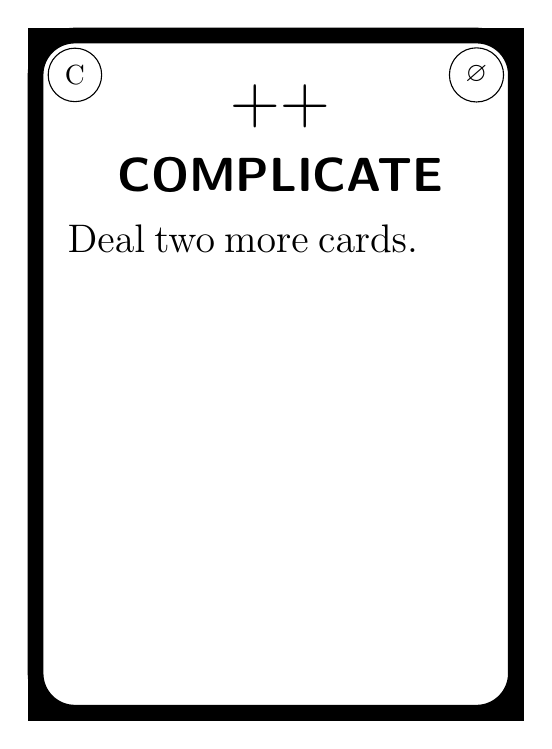
\begin{tikzpicture}
    \pgfmathsetmacro{\cardroundingradius}{5mm}
    \pgfmathsetmacro{\striproundingradius}{3mm}
    % \pgfmathsetmacro{\cardwidth}{5.9}
    % \pgfmathsetmacro{\cardheight}{9.2}
    \pgfmathsetmacro{\cardwidth}{6.1}  % Magic cards are 63x88mm
    \pgfmathsetmacro{\cardheight}{8.6}
    \pgfmathsetmacro{\stripwidth}{1.2}
    \pgfmathsetmacro{\strippadding}{0.1}
    \pgfmathsetmacro{\textpadding}{0.3}
    \pgfmathsetmacro{\ruleheight}{0.1}
    \providecommand{\stripfontsize}{\Huge}
    \providecommand{\captionfontsize}{\LARGE}
    \providecommand{\textfontsize}{\Large}
    \providecommand{\quotefontsize}{\small}
    \draw[fill=white, line width=2mm,rounded corners=\cardroundingradius] (0,0) rectangle (\cardwidth,\cardheight);
    \draw[line width=2mm] (0,0) rectangle (\cardwidth,\cardheight);
    \node[text width=(\cardwidth-\strippadding-2*\textpadding)*1cm,below right,inner sep=0] at (\strippadding+\textpadding,\cardheight-\textpadding) 
    { 
    \begin{center} {\fontsize{80pt}{60pt}\selectfont ++}\\\end{center}
\begin{center}
    {\captionfontsize \textsf{\textbf{COMPLICATE}}}\end{center}
        {\textfontsize Deal two more cards.}
        %\tikz{\fill (0,0) rectangle (\cardwidth-2*\strippadding-2*\textpadding,\ruleheight);}\\
        {\quotefontsize \textit{}}\\[-2\baselineskip]
    };
    \node[circle,draw,text=black](c) at (.5,\cardheight-.5){C};
    \node[circle,draw,text=black](c) at (\cardwidth-.5,\cardheight-.5){$\varnothing$};
    \end{tikzpicture}%
\hspace{1pt}%
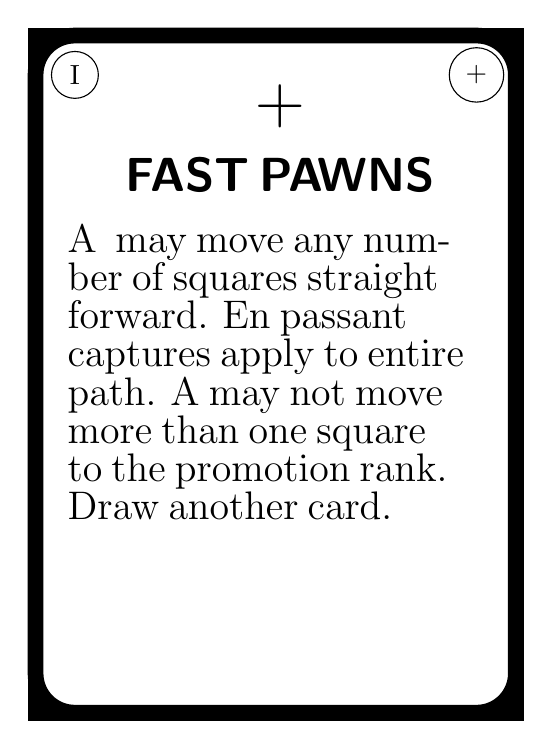
\begin{tikzpicture}
    \pgfmathsetmacro{\cardroundingradius}{5mm}
    \pgfmathsetmacro{\striproundingradius}{3mm}
    % \pgfmathsetmacro{\cardwidth}{5.9}
    % \pgfmathsetmacro{\cardheight}{9.2}
    \pgfmathsetmacro{\cardwidth}{6.1}  % Magic cards are 63x88mm
    \pgfmathsetmacro{\cardheight}{8.6}
    \pgfmathsetmacro{\stripwidth}{1.2}
    \pgfmathsetmacro{\strippadding}{0.1}
    \pgfmathsetmacro{\textpadding}{0.3}
    \pgfmathsetmacro{\ruleheight}{0.1}
    \providecommand{\stripfontsize}{\Huge}
    \providecommand{\captionfontsize}{\LARGE}
    \providecommand{\textfontsize}{\Large}
    \providecommand{\quotefontsize}{\small}
    \draw[fill=white, line width=2mm,rounded corners=\cardroundingradius] (0,0) rectangle (\cardwidth,\cardheight);
    \draw[line width=2mm] (0,0) rectangle (\cardwidth,\cardheight);
    \node[text width=(\cardwidth-\strippadding-2*\textpadding)*1cm,below right,inner sep=0] at (\strippadding+\textpadding,\cardheight-\textpadding) 
    { 
    \begin{center} {\fontsize{80pt}{60pt}\selectfont \Pawn+}\\\end{center}
\begin{center}
    {\captionfontsize \textsf{\textbf{FAST PAWNS}}}\end{center}
        {\textfontsize A \Pawn\ may move any number of squares straight forward. En passant captures apply to entire path. A \Pawn may not move more than one square to the promotion rank. Draw another card.}
        %\tikz{\fill (0,0) rectangle (\cardwidth-2*\strippadding-2*\textpadding,\ruleheight);}\\
        {\quotefontsize \textit{}}\\[-2\baselineskip]
    };
    \node[circle,draw,text=black](c) at (.5,\cardheight-.5){I};
    \node[circle,draw,text=black](c) at (\cardwidth-.5,\cardheight-.5){+};
    \end{tikzpicture}%
\hspace{1pt}%
\begin{tikzpicture}
    \pgfmathsetmacro{\cardroundingradius}{5mm}
    \pgfmathsetmacro{\striproundingradius}{3mm}
    % \pgfmathsetmacro{\cardwidth}{5.9}
    % \pgfmathsetmacro{\cardheight}{9.2}
    \pgfmathsetmacro{\cardwidth}{6.1}  % Magic cards are 63x88mm
    \pgfmathsetmacro{\cardheight}{8.6}
    \pgfmathsetmacro{\stripwidth}{1.2}
    \pgfmathsetmacro{\strippadding}{0.1}
    \pgfmathsetmacro{\textpadding}{0.3}
    \pgfmathsetmacro{\ruleheight}{0.1}
    \providecommand{\stripfontsize}{\Huge}
    \providecommand{\captionfontsize}{\LARGE}
    \providecommand{\textfontsize}{\Large}
    \providecommand{\quotefontsize}{\small}
    \draw[fill=white, line width=2mm,rounded corners=\cardroundingradius] (0,0) rectangle (\cardwidth,\cardheight);
    \draw[line width=2mm] (0,0) rectangle (\cardwidth,\cardheight);
    \node[text width=(\cardwidth-\strippadding-2*\textpadding)*1cm,below right,inner sep=0] at (\strippadding+\textpadding,\cardheight-\textpadding) 
    { 
    \begin{center} {\fontsize{80pt}{60pt}\selectfont \Knight\NoPawn}\\\end{center}
\begin{center}
    {\captionfontsize \textsf{\textbf{LEND ME YOUR HORSE}}}\end{center}
        {\textfontsize Non-pawn pieces protected by a knight may also act like a knight.}
        %\tikz{\fill (0,0) rectangle (\cardwidth-2*\strippadding-2*\textpadding,\ruleheight);}\\
        {\quotefontsize \textit{}}\\[-2\baselineskip]
    };
    \node[circle,draw,text=black](c) at (.5,\cardheight-.5){C};
    \node[circle,draw,text=black](c) at (\cardwidth-.5,\cardheight-.5){+};
    \end{tikzpicture}%
\hspace{1pt}%
\begin{tikzpicture}
    \pgfmathsetmacro{\cardroundingradius}{5mm}
    \pgfmathsetmacro{\striproundingradius}{3mm}
    % \pgfmathsetmacro{\cardwidth}{5.9}
    % \pgfmathsetmacro{\cardheight}{9.2}
    \pgfmathsetmacro{\cardwidth}{6.1}  % Magic cards are 63x88mm
    \pgfmathsetmacro{\cardheight}{8.6}
    \pgfmathsetmacro{\stripwidth}{1.2}
    \pgfmathsetmacro{\strippadding}{0.1}
    \pgfmathsetmacro{\textpadding}{0.3}
    \pgfmathsetmacro{\ruleheight}{0.1}
    \providecommand{\stripfontsize}{\Huge}
    \providecommand{\captionfontsize}{\LARGE}
    \providecommand{\textfontsize}{\Large}
    \providecommand{\quotefontsize}{\small}
    \draw[fill=white, line width=2mm,rounded corners=\cardroundingradius] (0,0) rectangle (\cardwidth,\cardheight);
    \draw[line width=2mm] (0,0) rectangle (\cardwidth,\cardheight);
    \node[text width=(\cardwidth-\strippadding-2*\textpadding)*1cm,below right,inner sep=0] at (\strippadding+\textpadding,\cardheight-\textpadding) 
    { 
    \begin{center} {\fontsize{80pt}{60pt}\selectfont \All}\\\end{center}
\begin{center}
    {\captionfontsize \textsf{\textbf{MOVE TWICE}}}\end{center}
        {\textfontsize You may move two different pieces as one action.}
        %\tikz{\fill (0,0) rectangle (\cardwidth-2*\strippadding-2*\textpadding,\ruleheight);}\\
        {\quotefontsize \textit{}}\\[-2\baselineskip]
    };
    \node[circle,draw,text=black](c) at (.5,\cardheight-.5){I};
    \node[circle,draw,text=black](c) at (\cardwidth-.5,\cardheight-.5){+};
    \end{tikzpicture}%
\hspace{1pt}%
\\[-.5\lineskip]
\begin{tikzpicture}
    \pgfmathsetmacro{\cardroundingradius}{5mm}
    \pgfmathsetmacro{\striproundingradius}{3mm}
    % \pgfmathsetmacro{\cardwidth}{5.9}
    % \pgfmathsetmacro{\cardheight}{9.2}
    \pgfmathsetmacro{\cardwidth}{6.1}  % Magic cards are 63x88mm
    \pgfmathsetmacro{\cardheight}{8.6}
    \pgfmathsetmacro{\stripwidth}{1.2}
    \pgfmathsetmacro{\strippadding}{0.1}
    \pgfmathsetmacro{\textpadding}{0.3}
    \pgfmathsetmacro{\ruleheight}{0.1}
    \providecommand{\stripfontsize}{\Huge}
    \providecommand{\captionfontsize}{\LARGE}
    \providecommand{\textfontsize}{\Large}
    \providecommand{\quotefontsize}{\small}
    \draw[fill=white, line width=2mm,rounded corners=\cardroundingradius] (0,0) rectangle (\cardwidth,\cardheight);
    \draw[line width=2mm] (0,0) rectangle (\cardwidth,\cardheight);
    \node[text width=(\cardwidth-\strippadding-2*\textpadding)*1cm,below right,inner sep=0] at (\strippadding+\textpadding,\cardheight-\textpadding) 
    { 
    \begin{center} {\fontsize{80pt}{60pt}\selectfont \Pawn}\\\end{center}
\begin{center}
    {\captionfontsize \textsf{\textbf{CHECKERS}}}\end{center}
        {\textfontsize Pawns move and capture like checkers. Captures (including multiple) are forced. Pawns may be promoted to any piece.}
        %\tikz{\fill (0,0) rectangle (\cardwidth-2*\strippadding-2*\textpadding,\ruleheight);}\\
        {\quotefontsize \textit{}}\\[-2\baselineskip]
    };
    \node[circle,draw,text=black](c) at (.5,\cardheight-.5){C};
    \node[circle,draw,text=black](c) at (\cardwidth-.5,\cardheight-.5){\diff};
    \end{tikzpicture}%
\hspace{1pt}%
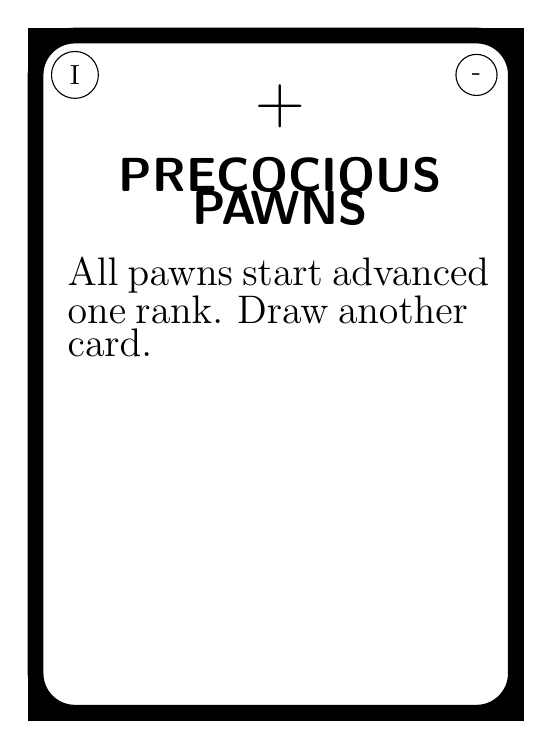
\begin{tikzpicture}
    \pgfmathsetmacro{\cardroundingradius}{5mm}
    \pgfmathsetmacro{\striproundingradius}{3mm}
    % \pgfmathsetmacro{\cardwidth}{5.9}
    % \pgfmathsetmacro{\cardheight}{9.2}
    \pgfmathsetmacro{\cardwidth}{6.1}  % Magic cards are 63x88mm
    \pgfmathsetmacro{\cardheight}{8.6}
    \pgfmathsetmacro{\stripwidth}{1.2}
    \pgfmathsetmacro{\strippadding}{0.1}
    \pgfmathsetmacro{\textpadding}{0.3}
    \pgfmathsetmacro{\ruleheight}{0.1}
    \providecommand{\stripfontsize}{\Huge}
    \providecommand{\captionfontsize}{\LARGE}
    \providecommand{\textfontsize}{\Large}
    \providecommand{\quotefontsize}{\small}
    \draw[fill=white, line width=2mm,rounded corners=\cardroundingradius] (0,0) rectangle (\cardwidth,\cardheight);
    \draw[line width=2mm] (0,0) rectangle (\cardwidth,\cardheight);
    \node[text width=(\cardwidth-\strippadding-2*\textpadding)*1cm,below right,inner sep=0] at (\strippadding+\textpadding,\cardheight-\textpadding) 
    { 
    \begin{center} {\fontsize{80pt}{60pt}\selectfont \Pawn+}\\\end{center}
\begin{center}
    {\captionfontsize \textsf{\textbf{PRECOCIOUS PAWNS}}}\end{center}
        {\textfontsize All pawns start advanced one rank. Draw another card.}
        %\tikz{\fill (0,0) rectangle (\cardwidth-2*\strippadding-2*\textpadding,\ruleheight);}\\
        {\quotefontsize \textit{}}\\[-2\baselineskip]
    };
    \node[circle,draw,text=black](c) at (.5,\cardheight-.5){I};
    \node[circle,draw,text=black](c) at (\cardwidth-.5,\cardheight-.5){-};
    \end{tikzpicture}%
\hspace{1pt}%
\begin{tikzpicture}
    \pgfmathsetmacro{\cardroundingradius}{5mm}
    \pgfmathsetmacro{\striproundingradius}{3mm}
    % \pgfmathsetmacro{\cardwidth}{5.9}
    % \pgfmathsetmacro{\cardheight}{9.2}
    \pgfmathsetmacro{\cardwidth}{6.1}  % Magic cards are 63x88mm
    \pgfmathsetmacro{\cardheight}{8.6}
    \pgfmathsetmacro{\stripwidth}{1.2}
    \pgfmathsetmacro{\strippadding}{0.1}
    \pgfmathsetmacro{\textpadding}{0.3}
    \pgfmathsetmacro{\ruleheight}{0.1}
    \providecommand{\stripfontsize}{\Huge}
    \providecommand{\captionfontsize}{\LARGE}
    \providecommand{\textfontsize}{\Large}
    \providecommand{\quotefontsize}{\small}
    \draw[fill=white, line width=2mm,rounded corners=\cardroundingradius] (0,0) rectangle (\cardwidth,\cardheight);
    \draw[line width=2mm] (0,0) rectangle (\cardwidth,\cardheight);
    \node[text width=(\cardwidth-\strippadding-2*\textpadding)*1cm,below right,inner sep=0] at (\strippadding+\textpadding,\cardheight-\textpadding) 
    { 
    \begin{center} {\fontsize{80pt}{60pt}\selectfont \Queen}\\\end{center}
\begin{center}
    {\captionfontsize \textsf{\textbf{NIGHT KING QUEEN}}}\end{center}
        {\textfontsize A Queen may only act like Knight or a King.}
        %\tikz{\fill (0,0) rectangle (\cardwidth-2*\strippadding-2*\textpadding,\ruleheight);}\\
        {\quotefontsize \textit{}}\\[-2\baselineskip]
    };
    \node[circle,draw,text=black](c) at (.5,\cardheight-.5){C};
    \node[circle,draw,text=black](c) at (\cardwidth-.5,\cardheight-.5){\diff};
    \end{tikzpicture}%
\hspace{1pt}%
\begin{tikzpicture}
    \pgfmathsetmacro{\cardroundingradius}{5mm}
    \pgfmathsetmacro{\striproundingradius}{3mm}
    % \pgfmathsetmacro{\cardwidth}{5.9}
    % \pgfmathsetmacro{\cardheight}{9.2}
    \pgfmathsetmacro{\cardwidth}{6.1}  % Magic cards are 63x88mm
    \pgfmathsetmacro{\cardheight}{8.6}
    \pgfmathsetmacro{\stripwidth}{1.2}
    \pgfmathsetmacro{\strippadding}{0.1}
    \pgfmathsetmacro{\textpadding}{0.3}
    \pgfmathsetmacro{\ruleheight}{0.1}
    \providecommand{\stripfontsize}{\Huge}
    \providecommand{\captionfontsize}{\LARGE}
    \providecommand{\textfontsize}{\Large}
    \providecommand{\quotefontsize}{\small}
    \draw[fill=white, line width=2mm,rounded corners=\cardroundingradius] (0,0) rectangle (\cardwidth,\cardheight);
    \draw[line width=2mm] (0,0) rectangle (\cardwidth,\cardheight);
    \node[text width=(\cardwidth-\strippadding-2*\textpadding)*1cm,below right,inner sep=0] at (\strippadding+\textpadding,\cardheight-\textpadding) 
    { 
    \begin{center} {\fontsize{80pt}{60pt}\selectfont \Bishop}\\\end{center}
\begin{center}
    {\captionfontsize \textsf{\textbf{CROWNED BISHOP}}}\end{center}
        {\textfontsize A bishop may also act like a King.}
        %\tikz{\fill (0,0) rectangle (\cardwidth-2*\strippadding-2*\textpadding,\ruleheight);}\\
        {\quotefontsize \textit{}}\\[-2\baselineskip]
    };
    \node[circle,draw,text=black](c) at (.5,\cardheight-.5){C};
    \node[circle,draw,text=black](c) at (\cardwidth-.5,\cardheight-.5){+};
    \end{tikzpicture}%
\hspace{1pt}%
\\[-.5\lineskip]
\begin{tikzpicture}
    \pgfmathsetmacro{\cardroundingradius}{5mm}
    \pgfmathsetmacro{\striproundingradius}{3mm}
    % \pgfmathsetmacro{\cardwidth}{5.9}
    % \pgfmathsetmacro{\cardheight}{9.2}
    \pgfmathsetmacro{\cardwidth}{6.1}  % Magic cards are 63x88mm
    \pgfmathsetmacro{\cardheight}{8.6}
    \pgfmathsetmacro{\stripwidth}{1.2}
    \pgfmathsetmacro{\strippadding}{0.1}
    \pgfmathsetmacro{\textpadding}{0.3}
    \pgfmathsetmacro{\ruleheight}{0.1}
    \providecommand{\stripfontsize}{\Huge}
    \providecommand{\captionfontsize}{\LARGE}
    \providecommand{\textfontsize}{\Large}
    \providecommand{\quotefontsize}{\small}
    \draw[fill=white, line width=2mm,rounded corners=\cardroundingradius] (0,0) rectangle (\cardwidth,\cardheight);
    \draw[line width=2mm] (0,0) rectangle (\cardwidth,\cardheight);
    \node[text width=(\cardwidth-\strippadding-2*\textpadding)*1cm,below right,inner sep=0] at (\strippadding+\textpadding,\cardheight-\textpadding) 
    { 
    \begin{center} {\fontsize{80pt}{60pt}\selectfont \Rook}\\\end{center}
\begin{center}
    {\captionfontsize \textsf{\textbf{CROWNED ROOK}}}\end{center}
        {\textfontsize A Rook may also act like a King.}
        %\tikz{\fill (0,0) rectangle (\cardwidth-2*\strippadding-2*\textpadding,\ruleheight);}\\
        {\quotefontsize \textit{}}\\[-2\baselineskip]
    };
    \node[circle,draw,text=black](c) at (.5,\cardheight-.5){C};
    \node[circle,draw,text=black](c) at (\cardwidth-.5,\cardheight-.5){+};
    \end{tikzpicture}%
\hspace{1pt}%
\begin{tikzpicture}
    \pgfmathsetmacro{\cardroundingradius}{5mm}
    \pgfmathsetmacro{\striproundingradius}{3mm}
    % \pgfmathsetmacro{\cardwidth}{5.9}
    % \pgfmathsetmacro{\cardheight}{9.2}
    \pgfmathsetmacro{\cardwidth}{6.1}  % Magic cards are 63x88mm
    \pgfmathsetmacro{\cardheight}{8.6}
    \pgfmathsetmacro{\stripwidth}{1.2}
    \pgfmathsetmacro{\strippadding}{0.1}
    \pgfmathsetmacro{\textpadding}{0.3}
    \pgfmathsetmacro{\ruleheight}{0.1}
    \providecommand{\stripfontsize}{\Huge}
    \providecommand{\captionfontsize}{\LARGE}
    \providecommand{\textfontsize}{\Large}
    \providecommand{\quotefontsize}{\small}
    \draw[fill=white, line width=2mm,rounded corners=\cardroundingradius] (0,0) rectangle (\cardwidth,\cardheight);
    \draw[line width=2mm] (0,0) rectangle (\cardwidth,\cardheight);
    \node[text width=(\cardwidth-\strippadding-2*\textpadding)*1cm,below right,inner sep=0] at (\strippadding+\textpadding,\cardheight-\textpadding) 
    { 
    \begin{center} {\fontsize{80pt}{60pt}\selectfont \Queen}\\\end{center}
\begin{center}
    {\captionfontsize \textsf{\textbf{REARGUARD}}}\end{center}
        {\textfontsize Whenever a Queen moves (not drop), it may summon a pawn to the square behind it.}
        %\tikz{\fill (0,0) rectangle (\cardwidth-2*\strippadding-2*\textpadding,\ruleheight);}\\
        {\quotefontsize \textit{}}\\[-2\baselineskip]
    };
    \node[circle,draw,text=black](c) at (.5,\cardheight-.5){C};
    \node[circle,draw,text=black](c) at (\cardwidth-.5,\cardheight-.5){+};
    \end{tikzpicture}%
\hspace{1pt}%
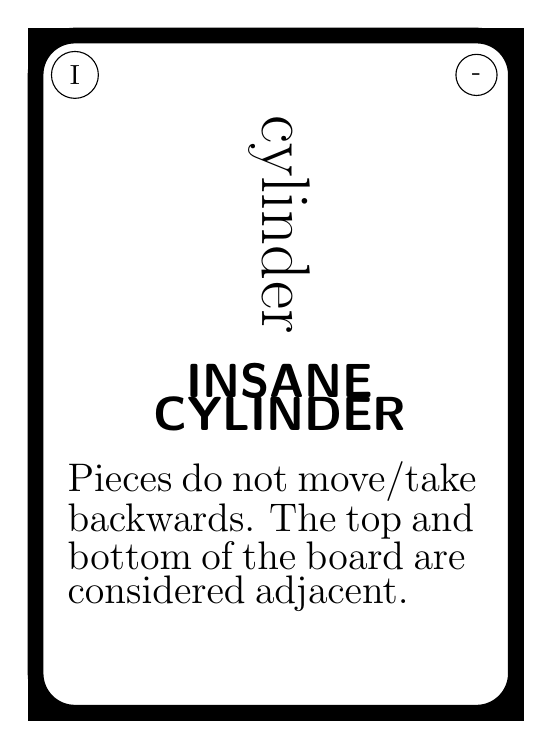
\begin{tikzpicture}
    \pgfmathsetmacro{\cardroundingradius}{5mm}
    \pgfmathsetmacro{\striproundingradius}{3mm}
    % \pgfmathsetmacro{\cardwidth}{5.9}
    % \pgfmathsetmacro{\cardheight}{9.2}
    \pgfmathsetmacro{\cardwidth}{6.1}  % Magic cards are 63x88mm
    \pgfmathsetmacro{\cardheight}{8.6}
    \pgfmathsetmacro{\stripwidth}{1.2}
    \pgfmathsetmacro{\strippadding}{0.1}
    \pgfmathsetmacro{\textpadding}{0.3}
    \pgfmathsetmacro{\ruleheight}{0.1}
    \providecommand{\stripfontsize}{\Huge}
    \providecommand{\captionfontsize}{\LARGE}
    \providecommand{\textfontsize}{\Large}
    \providecommand{\quotefontsize}{\small}
    \draw[fill=white, line width=2mm,rounded corners=\cardroundingradius] (0,0) rectangle (\cardwidth,\cardheight);
    \draw[line width=2mm] (0,0) rectangle (\cardwidth,\cardheight);
    \node[text width=(\cardwidth-\strippadding-2*\textpadding)*1cm,below right,inner sep=0] at (\strippadding+\textpadding,\cardheight-\textpadding) 
    { 
    \begin{center} {\fontsize{80pt}{60pt}\selectfont \rotatebox{-90}{\inlinegraphics{cylinder}}}\\\end{center}
\begin{center}
    {\captionfontsize \textsf{\textbf{INSANE CYLINDER}}}\end{center}
        {\textfontsize Pieces do not move/take backwards. The top and bottom of the board are considered adjacent.}
        %\tikz{\fill (0,0) rectangle (\cardwidth-2*\strippadding-2*\textpadding,\ruleheight);}\\
        {\quotefontsize \textit{}}\\[-2\baselineskip]
    };
    \node[circle,draw,text=black](c) at (.5,\cardheight-.5){I};
    \node[circle,draw,text=black](c) at (\cardwidth-.5,\cardheight-.5){-};
    \end{tikzpicture}%
\hspace{1pt}%
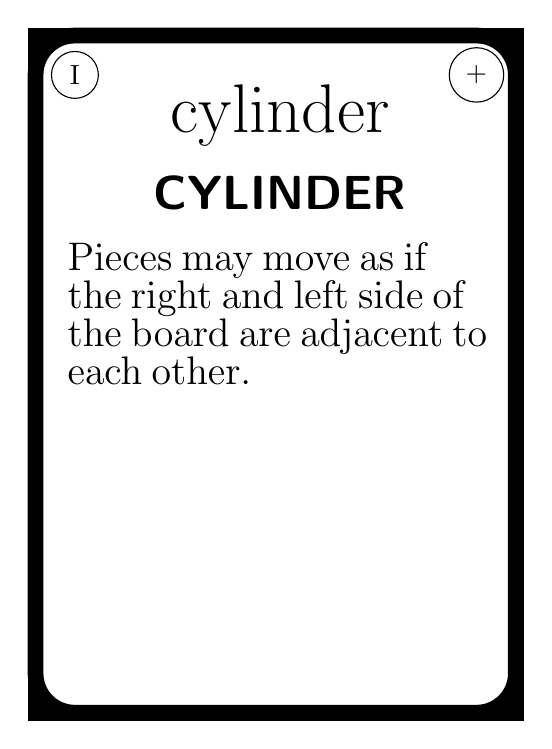
\begin{tikzpicture}
    \pgfmathsetmacro{\cardroundingradius}{5mm}
    \pgfmathsetmacro{\striproundingradius}{3mm}
    % \pgfmathsetmacro{\cardwidth}{5.9}
    % \pgfmathsetmacro{\cardheight}{9.2}
    \pgfmathsetmacro{\cardwidth}{6.1}  % Magic cards are 63x88mm
    \pgfmathsetmacro{\cardheight}{8.6}
    \pgfmathsetmacro{\stripwidth}{1.2}
    \pgfmathsetmacro{\strippadding}{0.1}
    \pgfmathsetmacro{\textpadding}{0.3}
    \pgfmathsetmacro{\ruleheight}{0.1}
    \providecommand{\stripfontsize}{\Huge}
    \providecommand{\captionfontsize}{\LARGE}
    \providecommand{\textfontsize}{\Large}
    \providecommand{\quotefontsize}{\small}
    \draw[fill=white, line width=2mm,rounded corners=\cardroundingradius] (0,0) rectangle (\cardwidth,\cardheight);
    \draw[line width=2mm] (0,0) rectangle (\cardwidth,\cardheight);
    \node[text width=(\cardwidth-\strippadding-2*\textpadding)*1cm,below right,inner sep=0] at (\strippadding+\textpadding,\cardheight-\textpadding) 
    { 
    \begin{center} {\fontsize{80pt}{60pt}\selectfont \inlinegraphics{cylinder}}\\\end{center}
\begin{center}
    {\captionfontsize \textsf{\textbf{CYLINDER}}}\end{center}
        {\textfontsize Pieces may move as if the right and left side of the board are adjacent to each other.}
        %\tikz{\fill (0,0) rectangle (\cardwidth-2*\strippadding-2*\textpadding,\ruleheight);}\\
        {\quotefontsize \textit{}}\\[-2\baselineskip]
    };
    \node[circle,draw,text=black](c) at (.5,\cardheight-.5){I};
    \node[circle,draw,text=black](c) at (\cardwidth-.5,\cardheight-.5){+};
    \end{tikzpicture}%
\hspace{1pt}%
\\[-.5\lineskip]
\begin{tikzpicture}
    \pgfmathsetmacro{\cardroundingradius}{5mm}
    \pgfmathsetmacro{\striproundingradius}{3mm}
    % \pgfmathsetmacro{\cardwidth}{5.9}
    % \pgfmathsetmacro{\cardheight}{9.2}
    \pgfmathsetmacro{\cardwidth}{6.1}  % Magic cards are 63x88mm
    \pgfmathsetmacro{\cardheight}{8.6}
    \pgfmathsetmacro{\stripwidth}{1.2}
    \pgfmathsetmacro{\strippadding}{0.1}
    \pgfmathsetmacro{\textpadding}{0.3}
    \pgfmathsetmacro{\ruleheight}{0.1}
    \providecommand{\stripfontsize}{\Huge}
    \providecommand{\captionfontsize}{\LARGE}
    \providecommand{\textfontsize}{\Large}
    \providecommand{\quotefontsize}{\small}
    \draw[fill=white, line width=2mm,rounded corners=\cardroundingradius] (0,0) rectangle (\cardwidth,\cardheight);
    \draw[line width=2mm] (0,0) rectangle (\cardwidth,\cardheight);
    \node[text width=(\cardwidth-\strippadding-2*\textpadding)*1cm,below right,inner sep=0] at (\strippadding+\textpadding,\cardheight-\textpadding) 
    { 
    \begin{center} {\fontsize{80pt}{60pt}\selectfont \NoKing}\\\end{center}
\begin{center}
    {\captionfontsize \textsf{\textbf{MOVE SWAP}}}\end{center}
        {\textfontsize Two friendly {\Sym\NoKing} may swap places if one can move to or take the other.}
        %\tikz{\fill (0,0) rectangle (\cardwidth-2*\strippadding-2*\textpadding,\ruleheight);}\\
        {\quotefontsize \textit{}}\\[-2\baselineskip]
    };
    \node[circle,draw,text=black](c) at (.5,\cardheight-.5){C};
    \node[circle,draw,text=black](c) at (\cardwidth-.5,\cardheight-.5){+};
    \end{tikzpicture}%
\hspace{1pt}%
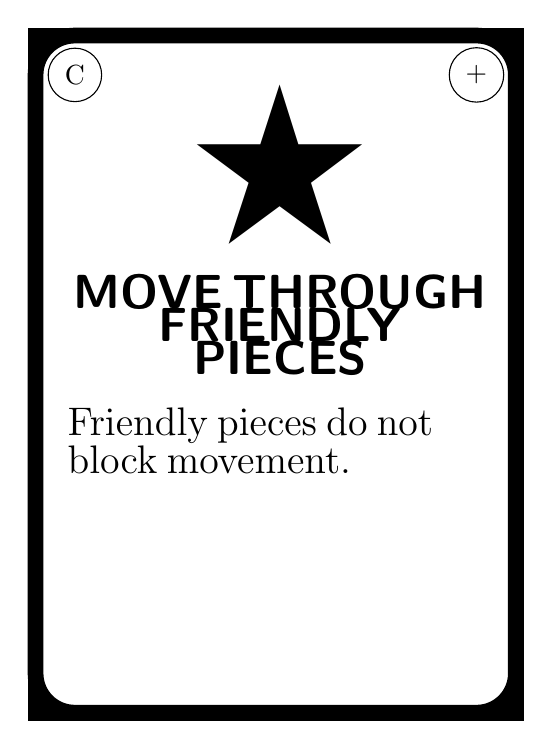
\begin{tikzpicture}
    \pgfmathsetmacro{\cardroundingradius}{5mm}
    \pgfmathsetmacro{\striproundingradius}{3mm}
    % \pgfmathsetmacro{\cardwidth}{5.9}
    % \pgfmathsetmacro{\cardheight}{9.2}
    \pgfmathsetmacro{\cardwidth}{6.1}  % Magic cards are 63x88mm
    \pgfmathsetmacro{\cardheight}{8.6}
    \pgfmathsetmacro{\stripwidth}{1.2}
    \pgfmathsetmacro{\strippadding}{0.1}
    \pgfmathsetmacro{\textpadding}{0.3}
    \pgfmathsetmacro{\ruleheight}{0.1}
    \providecommand{\stripfontsize}{\Huge}
    \providecommand{\captionfontsize}{\LARGE}
    \providecommand{\textfontsize}{\Large}
    \providecommand{\quotefontsize}{\small}
    \draw[fill=white, line width=2mm,rounded corners=\cardroundingradius] (0,0) rectangle (\cardwidth,\cardheight);
    \draw[line width=2mm] (0,0) rectangle (\cardwidth,\cardheight);
    \node[text width=(\cardwidth-\strippadding-2*\textpadding)*1cm,below right,inner sep=0] at (\strippadding+\textpadding,\cardheight-\textpadding) 
    { 
    \begin{center} {\fontsize{80pt}{60pt}\selectfont \ding{72}}\\\end{center}
\begin{center}
    {\captionfontsize \textsf{\textbf{MOVE THROUGH FRIENDLY PIECES}}}\end{center}
        {\textfontsize Friendly pieces do not block movement.}
        %\tikz{\fill (0,0) rectangle (\cardwidth-2*\strippadding-2*\textpadding,\ruleheight);}\\
        {\quotefontsize \textit{}}\\[-2\baselineskip]
    };
    \node[circle,draw,text=black](c) at (.5,\cardheight-.5){C};
    \node[circle,draw,text=black](c) at (\cardwidth-.5,\cardheight-.5){+};
    \end{tikzpicture}%
\hspace{1pt}%
\begin{tikzpicture}
    \pgfmathsetmacro{\cardroundingradius}{5mm}
    \pgfmathsetmacro{\striproundingradius}{3mm}
    % \pgfmathsetmacro{\cardwidth}{5.9}
    % \pgfmathsetmacro{\cardheight}{9.2}
    \pgfmathsetmacro{\cardwidth}{6.1}  % Magic cards are 63x88mm
    \pgfmathsetmacro{\cardheight}{8.6}
    \pgfmathsetmacro{\stripwidth}{1.2}
    \pgfmathsetmacro{\strippadding}{0.1}
    \pgfmathsetmacro{\textpadding}{0.3}
    \pgfmathsetmacro{\ruleheight}{0.1}
    \providecommand{\stripfontsize}{\Huge}
    \providecommand{\captionfontsize}{\LARGE}
    \providecommand{\textfontsize}{\Large}
    \providecommand{\quotefontsize}{\small}
    \draw[fill=white, line width=2mm,rounded corners=\cardroundingradius] (0,0) rectangle (\cardwidth,\cardheight);
    \draw[line width=2mm] (0,0) rectangle (\cardwidth,\cardheight);
    \node[text width=(\cardwidth-\strippadding-2*\textpadding)*1cm,below right,inner sep=0] at (\strippadding+\textpadding,\cardheight-\textpadding) 
    { 
    \begin{center} {\fontsize{80pt}{60pt}\selectfont \Queen}\\\end{center}
\begin{center}
    {\captionfontsize \textsf{\textbf{ARCHBISHOP}}}\end{center}
        {\textfontsize Queens move and take like Bishop+Knight. Fairy chess Archbishop.}
        %\tikz{\fill (0,0) rectangle (\cardwidth-2*\strippadding-2*\textpadding,\ruleheight);}\\
        {\quotefontsize \textit{}}\\[-2\baselineskip]
    };
    \node[circle,draw,text=black](c) at (.5,\cardheight-.5){F};
    \node[circle,draw,text=black](c) at (\cardwidth-.5,\cardheight-.5){\diff};
    \end{tikzpicture}%
\hspace{1pt}%
\begin{tikzpicture}
    \pgfmathsetmacro{\cardroundingradius}{5mm}
    \pgfmathsetmacro{\striproundingradius}{3mm}
    % \pgfmathsetmacro{\cardwidth}{5.9}
    % \pgfmathsetmacro{\cardheight}{9.2}
    \pgfmathsetmacro{\cardwidth}{6.1}  % Magic cards are 63x88mm
    \pgfmathsetmacro{\cardheight}{8.6}
    \pgfmathsetmacro{\stripwidth}{1.2}
    \pgfmathsetmacro{\strippadding}{0.1}
    \pgfmathsetmacro{\textpadding}{0.3}
    \pgfmathsetmacro{\ruleheight}{0.1}
    \providecommand{\stripfontsize}{\Huge}
    \providecommand{\captionfontsize}{\LARGE}
    \providecommand{\textfontsize}{\Large}
    \providecommand{\quotefontsize}{\small}
    \draw[fill=white, line width=2mm,rounded corners=\cardroundingradius] (0,0) rectangle (\cardwidth,\cardheight);
    \draw[line width=2mm] (0,0) rectangle (\cardwidth,\cardheight);
    \node[text width=(\cardwidth-\strippadding-2*\textpadding)*1cm,below right,inner sep=0] at (\strippadding+\textpadding,\cardheight-\textpadding) 
    { 
    \begin{center} {\fontsize{80pt}{60pt}\selectfont \Queen}\\\end{center}
\begin{center}
    {\captionfontsize \textsf{\textbf{CHANCELLOR}}}\end{center}
        {\textfontsize Queens move and take like Rook+Knight. Fairy chess Chancellor.}
        %\tikz{\fill (0,0) rectangle (\cardwidth-2*\strippadding-2*\textpadding,\ruleheight);}\\
        {\quotefontsize \textit{}}\\[-2\baselineskip]
    };
    \node[circle,draw,text=black](c) at (.5,\cardheight-.5){F};
    \node[circle,draw,text=black](c) at (\cardwidth-.5,\cardheight-.5){\diff};
    \end{tikzpicture}%
\hspace{1pt}%
\\[-.5\lineskip]

    \end{document}
    
